\documentclass[11pt]{article}
\usepackage{graphicx}
\usepackage{hyperref}
%\usepackage{appendix}
\usepackage{amsmath}
\usepackage{amsthm}
\usepackage{amssymb}
\usepackage{float}
\usepackage{commath}
%\usepackage{siunitx}
%\sisetup{detect-all}
\usepackage{listings}
\usepackage{color} %red, green, blue, yellow, cyan, magenta, black, white
\definecolor{mygreen}{RGB}{28,172,0} % color values Red, Green, Blue
\definecolor{mylilas}{RGB}{170,55,241}
\usepackage[a4paper,margin=20mm]{geometry}
\numberwithin{equation}{section}
\setlength{\parskip}{\baselineskip}
\setlength{\parindent}{0pt}
\hypersetup{
    colorlinks=true,
    linkcolor=magenta,
    filecolor=magenta,      
    urlcolor=magenta,
}
\urlstyle{same}
\begin{document}
\title{\textbf{UCL Mechanical Engineering 2020/2021}\\ENGF0004 Coursework 1}
\author{NCWT3}
\maketitle
\section{Question One}
\subsection*{a}
\begin{proof}
Left hand side:
\begin{gather}
	\sum_{n=0}^{\infty} \left(\frac{k-1}{k}\right)^n = 1 + \frac{k-1}{k} + \frac{\left(k-1\right)^2}{k^2} + ...\\
	a= 1, \ r = \frac{k-1}{k}
\end{gather}
$\frac{k-1}{k}$ is always less than 1 for $k > 1$. Hence:
\begin{gather}
	S_{\infty, LHS} = \frac{a}{1-r} = \frac{1}{1-\frac{k-1}{k}} = \frac{k}{k-k+1}\\
	S_{\infty, LHS} = k
\end{gather}
Right hand side:
\begin{gather}
	\left(k-1\right) \sum_{n=0}^{\infty} \left(\frac{1}{k}\right)^n = \left(k-1\right) \left[1 + \frac{1}{k} + \frac{1}{k^2} + ...\right]\\
	a = 1, \ r = \frac{1}{k}
\end{gather}
$\frac{1}{k}$ is always less than 1 for $k > 1$. Hence:
\begin{gather}
	S_{\infty,RHS} = \frac{k-1}{1 - \frac{1}{k}} = \frac{k\left(k-1\right)}{k-1}\\
	S_{\infty,RHS} = k\\
\end{gather}
LHS = RHS (for $k > 1$).
\end{proof}
\subsection*{b}
We are given:
\begin{align}
	f(x) &= \frac{x}{\sqrt{1-x}}\\
	f(x) &= x\left( 1 - x \right)^{-\frac{1}{2}}
\end{align}
Differentiating three times yields:
\begin{align}
	f'(x) &= \left(1 - x \right)^{-\frac{1}{2}} + \frac{x}{2} \left( 1-x\right)^{-\frac{3}{2}}\\
	f''(x) &= \frac{1}{2} \left( 1- x\right)^{-\frac{3}{2}} + \frac{1}{2} \left( 1- x\right)^{-\frac{3}{2}} + \frac{3x}{4} \left( 1-x \right)^{-\frac{5}{2}}\\
	&= \left( 1-x \right)^{-\frac{3}{2}} + \frac{3x}{4} \left( 1-x \right)^{-\frac{5}{2}} \\
	f'''(x) &= \frac{3}{2} \left( 1-x \right)^{-\frac{5}{2}} + \frac{3}{4} \left( 1-x \right)^{-\frac{5}{2}} + \frac{15x}{8} \left( 1-x \right)^{-\frac{7}{2}}\\
	&= \frac{9}{4} \left( 1-x \right)^{-\frac{5}{2}} + \frac{15x}{8} \left( 1-x \right)^{-\frac{7}{2}}
\end{align}
Inputting $x=0$:
\begin{align}
	f(0) &= 0 \cdot \left( 1 - 0 \right)^{-\frac{1}{2}} = 0\\
	f'(0) &= \left(1 - 0 \right)^{-\frac{1}{2}} + \frac{0}{2} \left( 1-0\right)^{-\frac{3}{2}} = 1\\
	f''(0) &= \left( 1-0 \right)^{-\frac{3}{2}} + \frac{3\cdot 0}{4} \left( 1-0 \right)^{-\frac{5}{2}} = 1\\
	f'''(0) &= \frac{9}{4} \left( 1-0 \right)^{-\frac{5}{2}} + \frac{15 \cdot 0}{8} \left( 1-0 \right)^{-\frac{7}{2}} = \frac{9}{4}
\end{align}
General form of Maclaurin series:
\begin{align}
	f(x) \approx f(0) + \frac{x}{1!}f'(0) + \frac{x^2}{2!}f''(0) + \frac{x^3}{3!}f'''(0) + ... \label{macser}
\end{align}
Inputting the above variables into Eq.\ref{macser}:
\begin{align}
	f(x) \approx x + \frac{x^2}{2} + \frac{3x^3}{8}	
\end{align}
\subsection*{c}
\subsubsection*{i}
We are given:
\begin{align}
E = \frac{kq}{x^2}
\end{align}
Sum of electric fields due to both charged particles is:
\begin{align}
	E &= \frac{ke}{\left( x-r \right)^2} - \frac{ke}{\left( x+r \right)^2}\\
	&= ke \left[ \frac{1}{x^2\left( 1 - \frac{r}{x} \right)^2} - \frac{1}{x^2\left( 1 + \frac{r}{x} \right)^2} \right]\\
	E&= \frac{ke}{x^2} \left[ \left( 1- \gamma \right)^{-2} - \left( 1 + \gamma\right)^{-2} \right]
\end{align}
Where $\gamma =\frac{r}{x}$.
\subsubsection*{ii}
Calculation of constants to be used in Maclaurin series expansion:
\begin{equation*}
	\begin{aligned}[c]
		f(\gamma) &= \left( 1 - \gamma \right)^{-2}\\
		f'(\gamma) &= 2\left(1-\gamma\right)^{-3}\\
		f''(\gamma) &= 6\left(1-\gamma\right)^{-4}\\
		f'''(\gamma) &= 24\left(1-\gamma\right)^{-5}
	\end{aligned}
	\makebox[2cm]{}
	\begin{aligned}[c]
		f(0) &= 1\\
		f'(0) &= 2\\
		f''(0) &= 6\\
		f'''(0) &= 24\\
	\end{aligned}
\end{equation*}
\begin{equation*}
	\begin{aligned}[c]
		g(\gamma) &= \left( 1 + \gamma \right)^{-2}\\
		g'(\gamma) &= -2\left(1+\gamma\right)^{-3}\\
		g''(\gamma) &= 6\left(1+\gamma\right)^{-4}\\
		g'''(\gamma) &= -24\left(1+\gamma\right)^{-5}
	\end{aligned}
	\makebox[2cm]{}
	\begin{aligned}[c]
		g(0) &= 1\\
		g'(0) &= -2\\
		g''(0) &= 6\\
		g'''(0) &= -24\\
	\end{aligned}
\end{equation*}
Inputting the above variables into Eq.\ref{macser}:
\begin{align}
	f(\gamma) &\approx 1 + \frac{2 \gamma}{1!} + \frac{6\gamma^2}{2!} + \frac{24\gamma^3}{3!} + ...\\
	f(\gamma) &\approx 1 + 2\gamma+ 3\gamma^2 + 4\gamma^3 \\ 
	g(\gamma) &\approx 1 - \frac{2 \gamma}{1!} + \frac{6\gamma^2}{2!} - \frac{24\gamma^3}{3!} + ...\\
	g(\gamma) &\approx 1 - 2\gamma + 3\gamma^2 - 4\gamma^2
\end{align}
Substitution:
\begin{align}
	E &\approx \frac{ke}{x^2} \left[ f(\gamma) - g(\gamma)\right]\\
	&\approx \frac{ke}{x^2} \left[ 1 + 2\gamma + 3\gamma^2 + 4\gamma^3 - 1 + 2\gamma - 3\gamma^2 + 4\gamma^3 \right]\\
	&\approx \frac{ke}{x^2}\left[ 4\gamma + 8\gamma^3 \right]\\
	E &\approx \frac{4ke}{x^2}\left[ \gamma + 2\gamma^3 \right]
\end{align}
\subsubsection*{iii}
$y = 0.01$. Exact:
\begin{align}
	E_E &= \frac{ke}{x^2} \left[\left(1-0.01\right)^{-2}-\left(1+0.01\right)^{-2}\right]\\
	E_E &= \frac{ke}{x^2} \left[0.0400080012\right]\\
\end{align}
Approximation:
\begin{align}
	E_A &= \frac{4ke}{x^2} \left[0.01 + 2\left(0.01\right)^3\right]\\
	E_A &= \frac{ke}{x^2} \left[0.040008\right]
\end{align}
Percentage error:
\begin{align}
	\frac{E_E - E_A}{E_E} \cdot 100 = \frac{0.0400080012 - 0.040008}{0.0400080012} \cdot 100 = 3.0\times 10^6\, \% \textrm{ error (2sf)}
\end{align}
\subsection*{d}
We are given:
\begin{align}
	y'' - 2y' + y = te^t\\
	y(0) = 0, \ y'(0)=1
\end{align}
Laplace transformation (from tables):
\begin{gather}
	\mathcal{L} \{ y''\} - 2\mathcal{L} \{ y'\} + \mathcal{L} \{ y\} = \mathcal{L} \{te^t \}\\
	s^2 Y(s) - sy(0) - y'(0) - 2\left(sY(s) - y(0)\right) + Y(s) = \frac{1!}{\left(s-1\right)^2}\\
	s^2 Y(s) -1 -2(sY(s) - 1) + Y(s) = \frac{1}{\left(s-1\right)^2}\\
	Y(s)\left[s^2-2s+1\right] -1 = \frac{1}{\left(s-1\right)^2}\\
	Y(s) = \frac{1}{\left(s-1\right)^2} + 1\\
	Y(s) = \frac{1}{\left(s-1\right)^4} + \frac{1}{\left(s-1\right)^2}
\end{gather}
Returning to time domain. From tables:
\begin{gather}
	L^{-1}\left[\frac{n!}{\left(s-a\right)^n}\right] = t^ne^{at}\\
	L^{-1}\left[\frac{1}{\left(s-1\right)^2}\right] = te^t\\
	\frac{1}{6}L^{-1}\left[\frac{3!}{\left(s-1\right)^2}\right] = \frac{1}{6}t^3e^t\\
	y(t) = \frac{1}{6}t^3e^t + te^t
\end{gather}
\subsection*{e}
\subsubsection*{i}
$a =1 \therefore -3 \leq t \leq 3$. Sketch:
\begin{figure}[H]
	\centering
	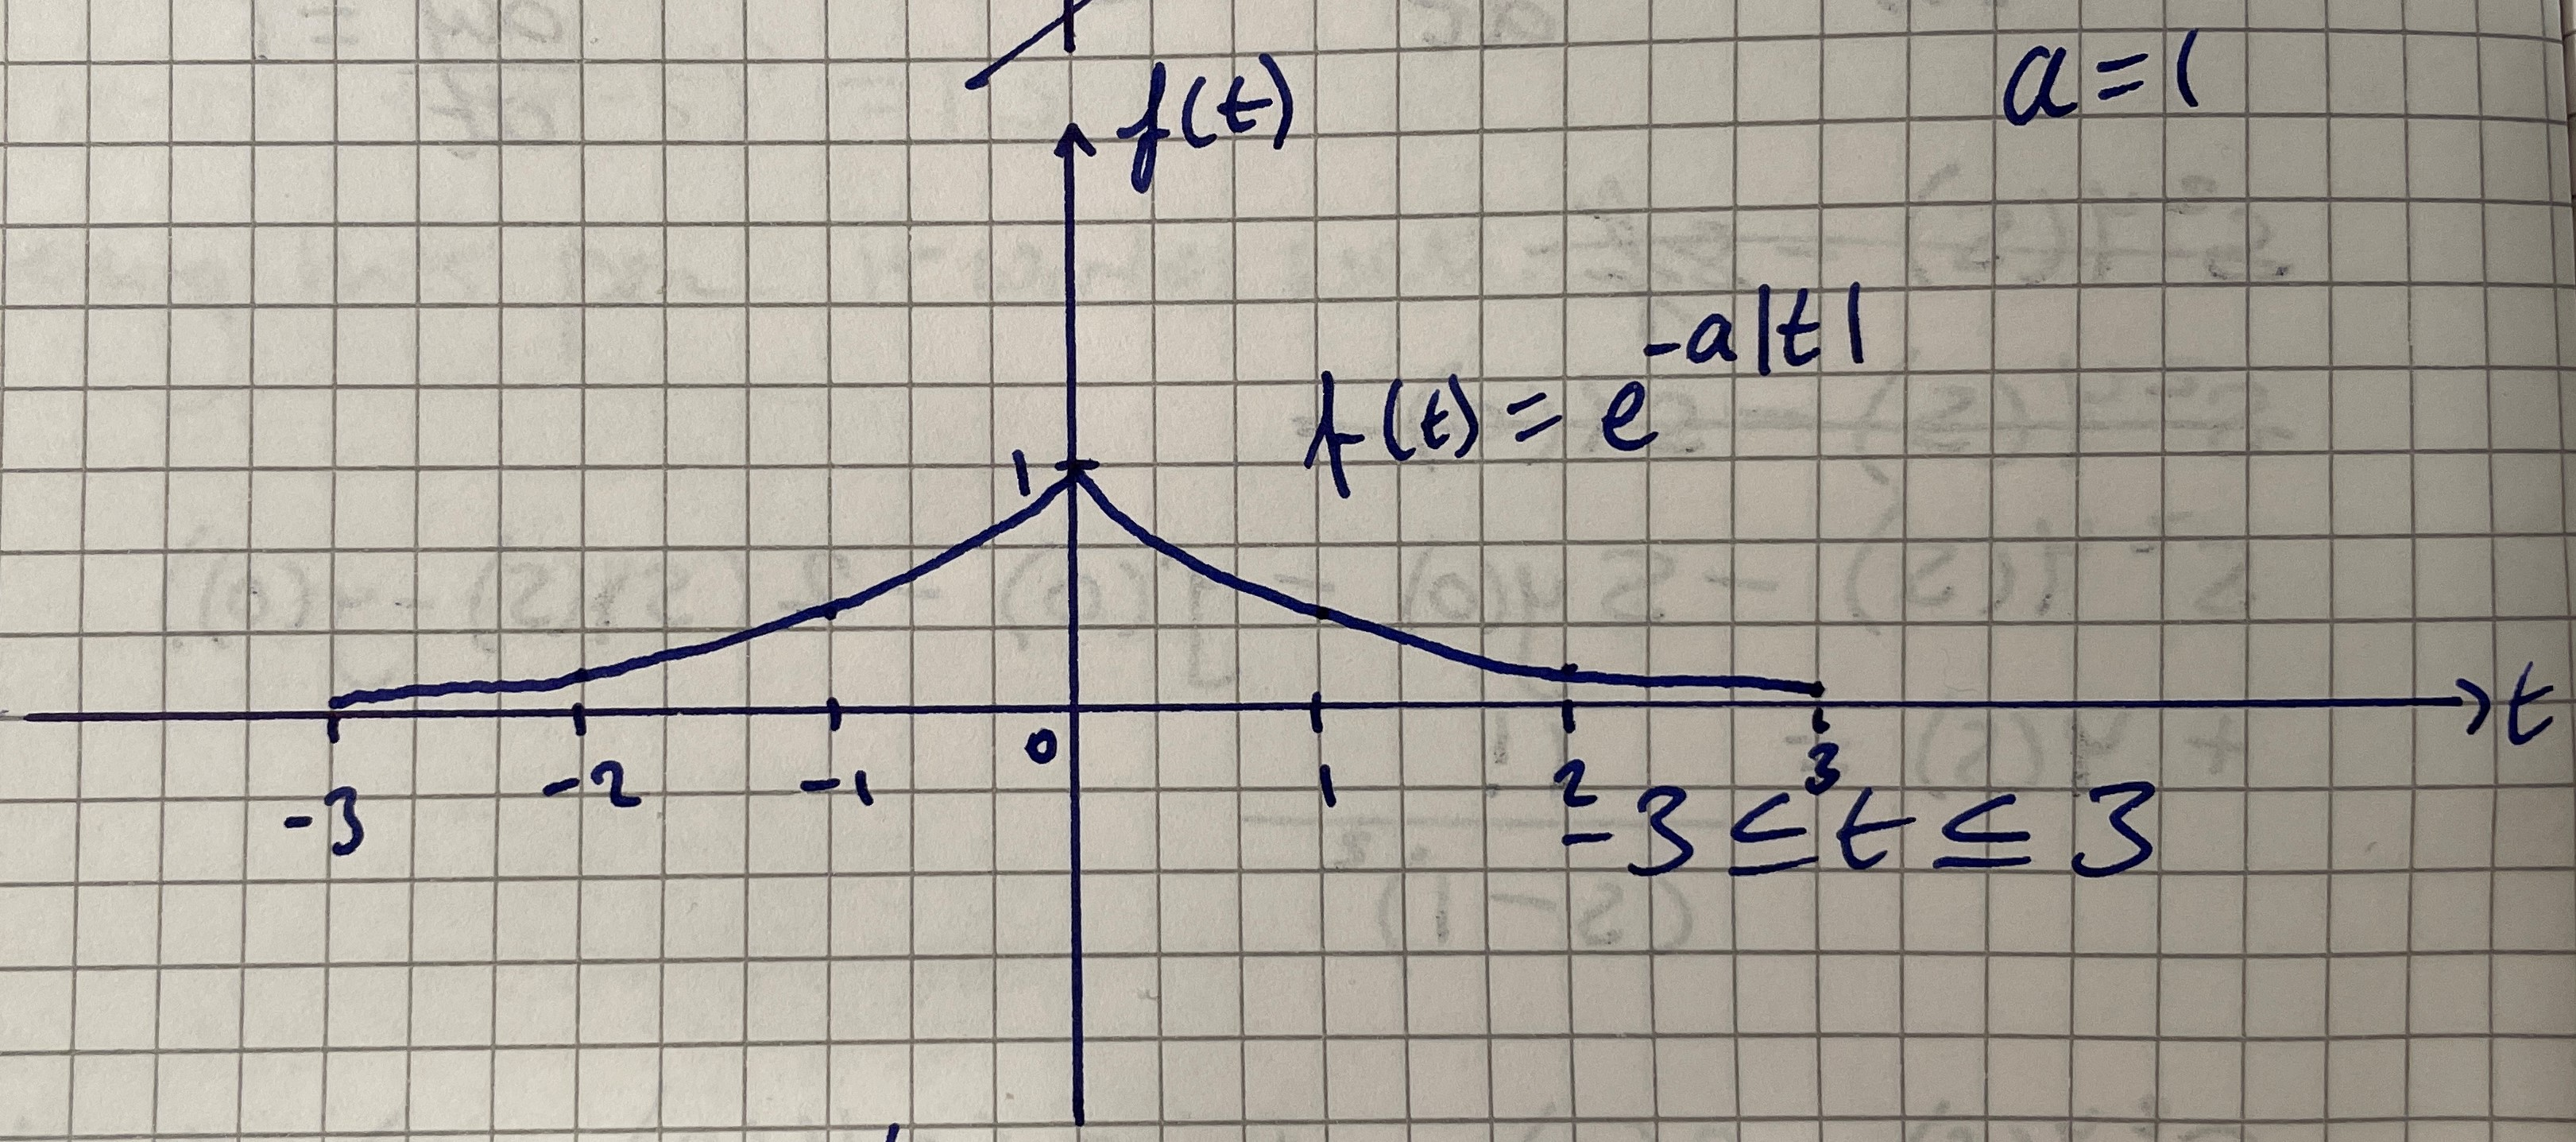
\includegraphics[width = 0.7\textwidth]{./img/q1ei.JPG}
	\caption{}
\end{figure}
\subsubsection*{ii}
Let $z = \infty$.
\begin{align}
	F(u) &= \lim_{z\rightarrow \infty} \int_{t=-z}^{0}e^{at}e^{-j2\pi u t}  \,\dif t + \lim_{z\rightarrow \infty}\int_{t=0}^{z} e^{-at} e^{-j2\pi u t}\,\dif t\\
	&= \lim_{z\rightarrow \infty} \int_{t=-\infty}^{0}e^{t(a - j2\pi u)}  \,\dif t + \lim_{z\rightarrow \infty} \int_{t=0}^{\infty} e^{-t(a + j2\pi u)}\,\dif t\\
	F(u) &= \lim_{z\rightarrow \infty} \left[ \left. \frac{1}{\left(a - j2\pi u\right)}e^{t\left(a - j2\pi u\right)} \right|_{t = -z}^0 \right] + \lim_{z\rightarrow \infty} \left[ \left. \frac{1}{-\left(a + j2\pi u\right)}e^{-t\left(a + j2\pi u\right)} \right|_{t=0}^z \right]
\end{align}
Applying limits:
\begin{align}
	\lim_{z\rightarrow \infty} \left[ \frac{1}{\left(a - j2\pi u\right)} \left[ 1 - e^{-z\left(a - j2\pi u\right)} \right] \right] = \left[ \frac{1}{\left(a - j2\pi u\right)} \left[ 1 - 0 \right] \right] &= \frac{1}{a - j2\pi u}\\
	\lim_{z\rightarrow \infty} \left[ \frac{-1}{\left(a + j2\pi u\right)} \left[ e^{-z\left( a + j2\pi u\right)} -1 \right]\right] = \left[ \frac{-1}{\left(a + j2\pi u\right)} \left[ 0 -1 \right]\right] &= \frac{1}{a + j2\pi u}
\end{align}
\begin{align}
	F(u) &= \frac{1}{a - j2\pi u} + \frac{1}{a + j2\pi u}\\
	&= \frac{a + j2\pi u + a - j2\pi u}{a^2 + 4\pi^2 u^2}\\
	F(u) &= \frac{2a}{a^2 + 4\pi^2u^2}
\end{align}
\subsubsection*{iii}
Substituting $\omega = 2\pi u$, $\omega^2 = 4\pi^2 u^2$:
\begin{align}
	F(\omega) = \frac{2a}{a^2 + \omega^2}
\end{align}
\begin{figure}[H]
	\centering
	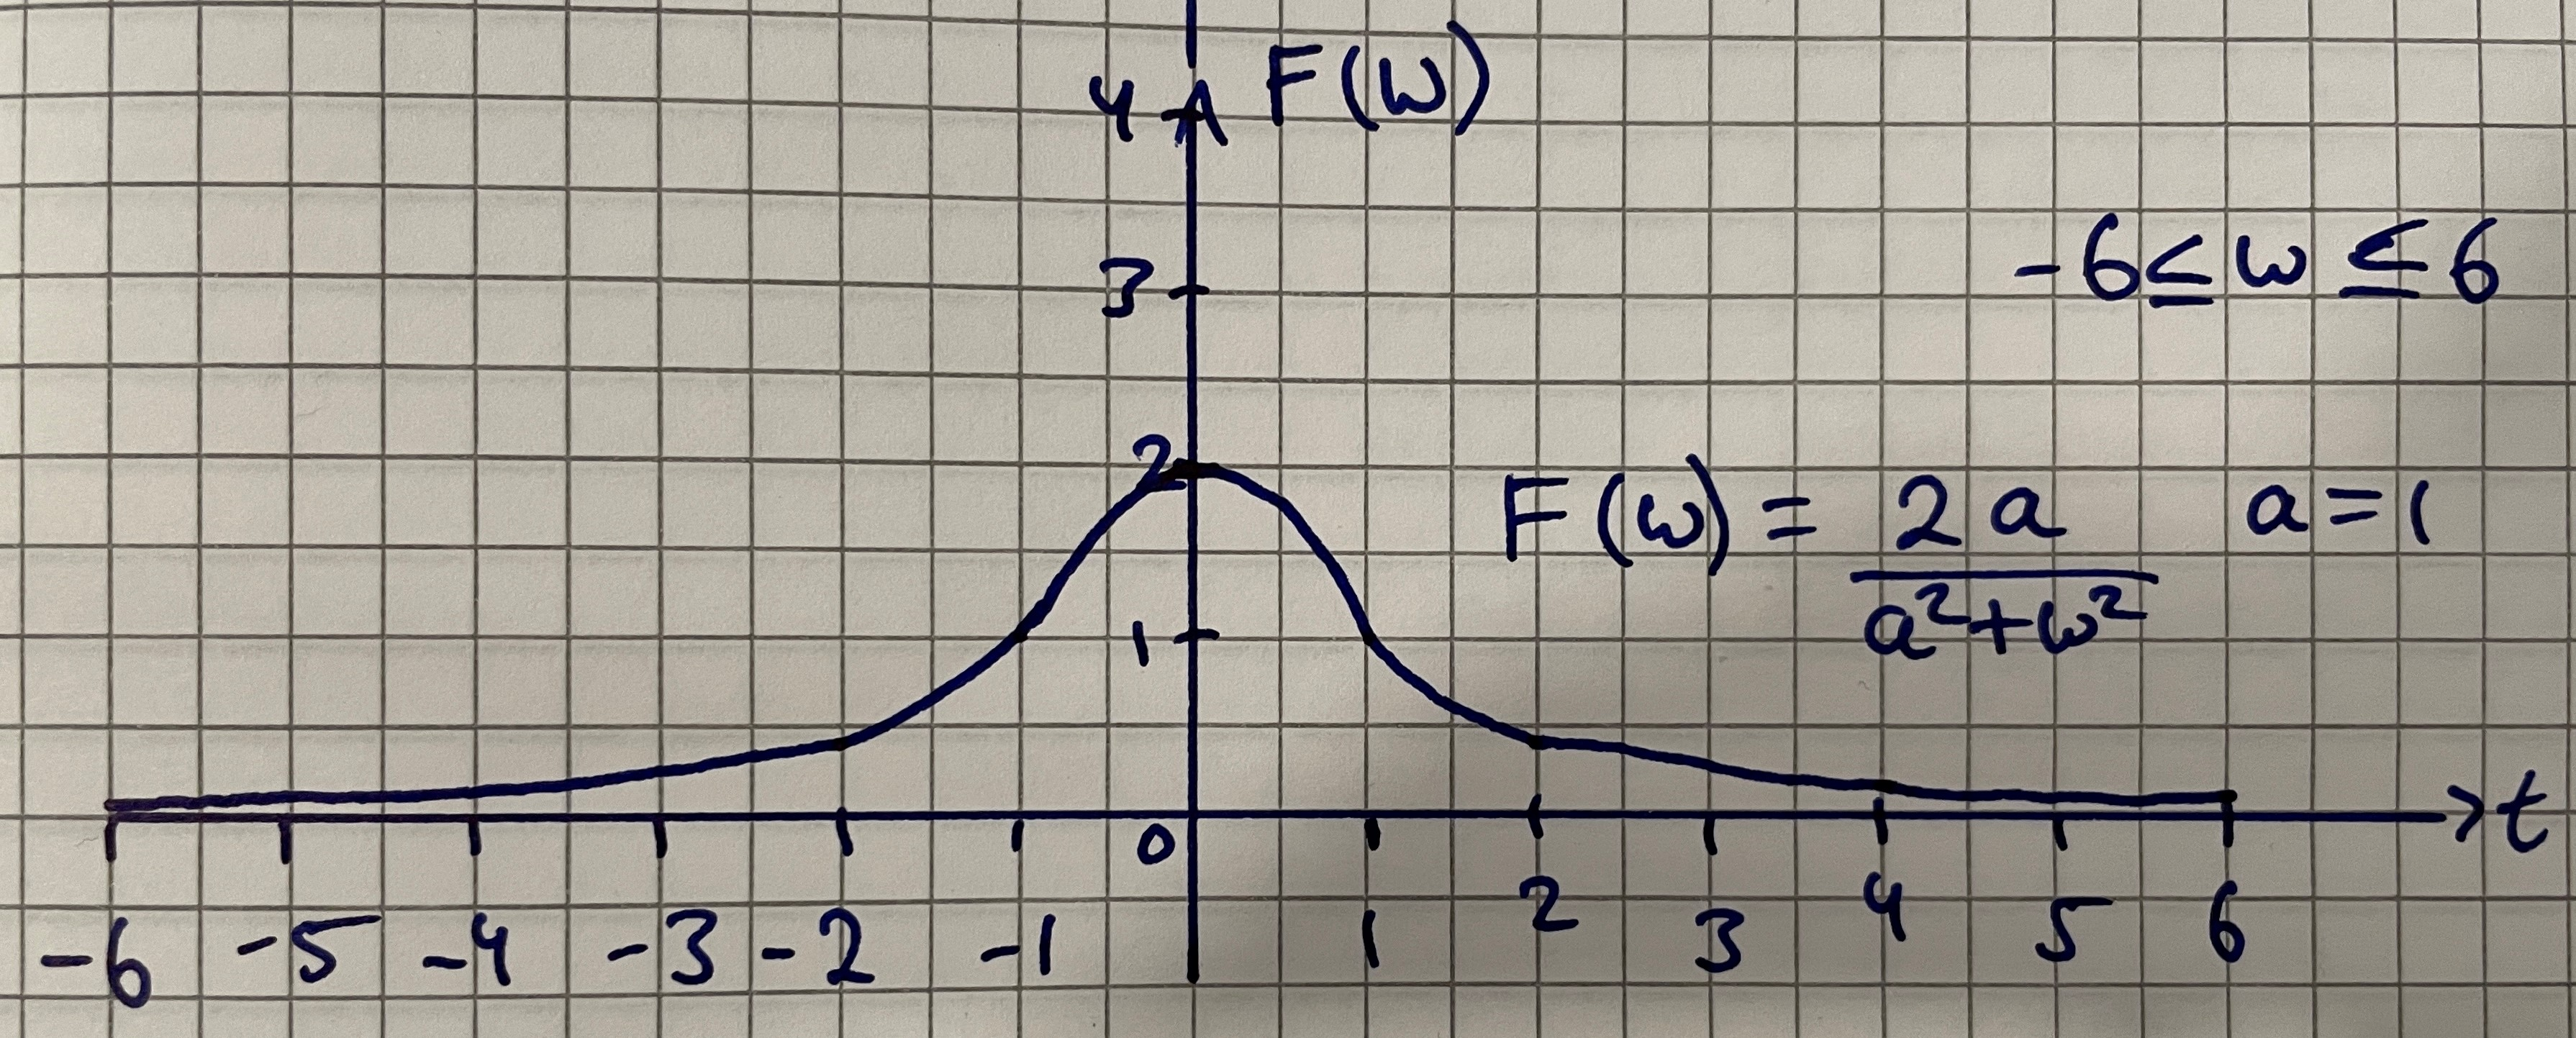
\includegraphics[width = 0.7\textwidth]{./img/q1eiii.JPG}
	\caption{}
\end{figure}
\subsubsection*{iv}
Full width at half maximum of $F\left(u\right)$ can be calculated as:
\begin{align}
	\frac{1}{2} &= e^{-at}\\
	\ln \left(\frac{1}{2}\right) &= -at\\
	-\ln \left(2\right) &= at\\
	t &= \frac{\ln \left( 2 \right)}{a} \rightarrow \textrm{HWHM}\\
	\therefore \textrm{FWHM} &= \frac{2\ln \left( 2 \right)}{a}
\end{align}
Full width at half maximum of $F\left(\omega\right)$ can be calculated as:
\begin{align}
	\frac{1}{2}\cdot\frac{2}{a} &= 2\frac{a}{a^2 + \omega^2}\\
	\frac{1}{a} &= \frac{2a}{a^2 + \omega^2}\\
	\omega^2 + a^2 &= 2a^2\\
	\omega &= a \rightarrow \textrm{HWHM}\\
	\therefore \textrm{FWHM} &= 2a 
\end{align}
\subsubsection*{v}
Product of FWHMs:
\begin{align}
	2a\cdot \frac{2\ln\left(2\right)}{a} &= 4\ln\left(2\right)
\end{align}
The product has no $a$ term, thus there is no dependence on the parameter.
\section{Question Two}
\subsection*{a}
\subsubsection*{i}
\begin{align}
	\frac{\partial u}{\partial t} = k \frac{\partial^2 u}{\partial x^2}\label{PDEq2ai}
\end{align}
We know that $u(x,t) = X(x)T(t)$. Substituting:
\begin{gather}
	X\left(x\right) T'\left(t\right) = kX''\left(x\right)T\left(t\right)\\
	\frac{T'\left(t\right)}{kT\left(t\right)} = \frac{X''\left(x\right)}{X\left(x\right)} = \mu \\
	X''\left(x\right) = \mu X\left(x\right)\\
	T'\left(t\right) = \mu k T\left(t\right)
\end{gather}
where $\mu$ is an arbitrary constant. If we define $\mu$ as negative then we obtain:
\begin{align}
	-X''\left(x\right) = \mu X\left(x\right)\\
	T'\left(t\right) = -\mu k T\left(t\right)
\end{align}
\subsubsection*{ii}
$\mu$ can be either positive, zero or negative. Let us consider these cases. 

\textbf{Case 1: positive constant $\mu = \lambda^2 > 0$}
\begin{align}
	\frac{X''\left(x\right)}{X\left(x\right)} &= \lambda^2\\
	X''\left(x\right) - \lambda^2X\left(x\right) &= 0 
\end{align}
Auxiliary equation:
\begin{gather}
	m^2 - \lambda^2 = 0\\
	m_1 = \lambda, \ m_2 = -\lambda
\end{gather}
Real and distinct roots. Hence:
\begin{align}
	X(x) = Ae^{\lambda x} + Be^{-\lambda x}
\end{align}
Applying boundary conditions for $x$. Applying $u\left(0,t\right) = 0$ implies $X(0)T(t) = 0$. Substituting $x=0$ in $X(x)$ gives:
\begin{gather}
	X(0) = A + B\\
	\left(A+B\right)T(t) = 0\\
	T(t) = 0 \textrm{ or } A + B =0
\end{gather}
$T(t) = 0$ leads to a trivial solution of $u(x,t) = X(x)T(t) = 0$. We also have $A + B = 0$ or $A = - B$:
\begin{gather}
	X(x) = A\left(e^{\lambda x} - e^{-\lambda x}\right)
\end{gather}
Applying $u(l,t) = 0$ implies $X(l)T(t) = 0$. Substituting $x=l$ in $X(x)$ gives: $X(l) = A\left(e^{\lambda l} - e^{-\lambda l}\right)$
\begin{gather}
	A\left(e^{\lambda l} - e^{-\lambda l}\right)T(t) = 0\\
	A = 0, \ T(t) = 0, \textrm{ or } e^{\lambda l} - e^{-\lambda l} = 0
\end{gather}
$T(t) = 0$ and $A=0$ both will lead to a trivial solution of $u(x,t) = X(x)T(t) =0$. $e^{\lambda l} - e^{-\lambda l} = 0$ is only true if $\lambda = 0$. However, the assumption in this case is $\lambda = \sqrt{\mu}$ where $\mu$ is a positive constant ($\lambda > 0$). Therefore, this boundary condition cannot be met and there are no useful solutions from Case 1.

\textbf{Case 2: zero constant $\lambda = 0$}
\begin{gather}
	\frac{X''(x)}{X(x)} = \lambda = 0\\
	X''(x) = 0\\
	\int X''(x) \dif x = \int \dif x\\
	X'(x) = C\\
	\int X'(x) = \int C \dif x\\
	X(x) = Cx + D
\end{gather}
where $C$ and $D$ are constants of integration. Applying boundary conditions for $x$. Applying $u(0,t) = 0$ implies $X(0)T(t) = 0$. Substituting $x=0$ in $X(x)$ gives:
\begin{gather}
	X(0) = D\\
	DT(t) = 0
	T(t) = 0 \textrm{ or } D = 0
\end{gather}
$T(t) = 0$ will lead to a trivial solution of $u(x,t) = X(x)T(t) =0$. Therefore, $D=0$.
\begin{align}
	X(x) = Cx
\end{align}
Applying $u(l,t) = 0$ implies $X(l)X(t) = 0$. Substituting $x=l$ in $X(x)$ gives:
\begin{gather}
	X(l) = Cl\\
	ClT(t) = 0\\
	T(t) = 0 \textrm{ or } C = 0
\end{gather}
$T(t) = 0$ and $C=0$ both will lead to a trivial solution of $u(x,t) = X(x)T(t) =0$. Case 2 only produces the trivial solution of $u(x,t) = X(x)T(t) =0$ and does not produce any useful solutions. 

\textbf{Case 3: negative constant $\mu = \lambda^2 < 0$}
\begin{align}
	\frac{X''\left(x\right)}{X\left(x\right)} &= -\lambda^2\\
	X''\left(x\right) + \lambda^2X\left(x\right) &= 0 
\end{align}
Auxiliary equation:
\begin{gather}
	m^2 + \lambda^2 = 0\\
	m_1 = i\lambda, \ m_2 = -i\lambda
\end{gather}
Complex and distinct roots. Hence:
\begin{align}
	X(x) = Ce^{i\lambda x} + De^{-i\lambda x}
\end{align}
Using Euler's formula and expanding:
\begin{align}
	X(x) = A\cos\left(\lambda x\right) + B\sin\left(\lambda x\right)
\end{align}
where $A = C +D$ and $B = i\left(C-D\right)$. Applying boundary conditions for $x$. Applying $u(0,t) = 0$ implies $X(0)T(t) = 0$. Substituting $x=0$ in $X(x)$ gives:
\begin{gather}
	X(0) = A\\
	AT(t) = 0\\
	T(t) = 0, \ A = 0
\end{gather}
$T(t) = 0$ will lead to a trivial solution of $u(x,t) = X(x)T(t) = 0$. Therefore, $A = 0$
\begin{align}
	X(x) = B\sin\left(\lambda x\right)
\end{align}
Applying $u(l,t) = 0$ implies $X(l)T(t) = 0$. Substituting $x=l$ in $X(x)$ gives:
\begin{gather}
	X(l) = B\sin\left(\lambda l\right)\\
	D\sin\left(\lambda l\right)T(t) = 0\\
	T(t) = 0, \ B = 0 \textrm{ or } \sin\left(\lambda l\right) = 0
\end{gather}
$T(t) = 0$ will lead to a trivial solution of $u(x,t) = X(x)T(t) = 0$. $B=0$ will lead to a trivial solution of $u(x,t) = X(x)T(t) = 0$. 
\begin{gather}
	\sin\left(\lambda l\right) = 0\\
	\lambda l = n\pi \textrm{ for } n = 1,2,3,...\\
	\lambda_n = \frac{n\pi}{l}\\
	\mu_n = -\left(\lambda_n\right)^2 = -\left(\frac{n\pi}{l}\right)^2
\end{gather}
We can denote $B_n$ to represent the various constants that correspond to each value of $\mu$. Therefore:
\begin{align}
	X(x) = B_n \sin\left(\frac{n\pi x}{l}\right) \textrm{ for } n=1,2,3,...
\end{align}
ODE in $T(t)$:
\begin{align}
	\frac{T'(t)}{kT(t)} = \mu_n = -\left(\lambda_n^2\right)\\
	\int \left(\frac{T'(t)}{T(t)}\right) \dif t = \int \left(\mu_n k\right) \dif t
\end{align}
In $T(t) = \mu_n kt + d_n$ where $d_n$ is a constant of integration for the differing values of each value of $\mu_n$.
\begin{align}
	T(t) = A_n e^{-\lambda_n^2 kt} 
\end{align}
where $A_n = e^{d_n}$. Therefore:
\begin{align}
	u(x,t) = X(x)T(t) = c_n e^{-\lambda_n^2 kt}\sin\left(\frac{n\pi x}{l}\right)
\end{align}
where $c_n = A_n B_n$. Let $u_n(x,t) e^{-\lambda_n^2 kt}\sin\left(\frac{n\pi x}{l}\right)$. The principle of superposition gives:
\begin{align}
	u(x,t) = \sum_{n=1}^{\infty} c_n u_n(x,t)
\end{align}
Applying the initial condition $u(x,0) = f(x)$ $0\leq x\leq l$. We have:
\begin{align}
	f(x) = \sum_{n=1}^{\infty} c_n \sin\left(\frac{n\pi x}{l}\right)
\end{align}
\subsubsection*{iii}
Using Fourier series:
\begin{align}
	c_n = \frac{2}{l}\int_{0}^{l} \left(f(x)\sin\left(n\pi x\right)\right) \,\dif x 
\end{align}
We are given:
\begin{align}
	u(x,0) = f(x) = x^2, \ 0 \leq x \leq l\\
	u(0,t) = u(l,t) = 0, \ t > 0\\
\end{align}
Let $a = \frac{n\pi}{l}$. Substituting the above into Fourier:
\begin{align}
	c_n = \frac{2}{l} \int_{0}^{l} \left( x^2 \sin\left(a x\right) \right) \,\dif x \\
\end{align}
Integration by parts once. $u = x^2$, $u' = 2x$, $v = -\frac{\cos\left(a x\right)}{n\pi}$ and $v' = \sin\left(a x\right)$.
\begin{align}
	c_n = \frac{2}{l}\left[ -\frac{x^2 \cos\left(a x\right)}{a} + \frac{2}{a}\int_{0}^{l} \left(x\cos\left(a x\right)\right) \,\dif x \right]_0^l
\end{align} 
Integration by parts twice. $u = x$, $u = 1$, $v= \frac{\sin\left(a x\right)}{a}$ and $v' = \cos\left(a x\right)$.
\begin{align}
	c_n &= \frac{2}{l}\left[ -\frac{x^2 \cos\left(a x\right)}{a} + \frac{2}{a}\left[ \frac{x\sin\left(a x\right)}{a} - \frac{1}{a} \int_{0}^{l} \left(\sin\left(a x\right)\right) \,\dif x \right]_0^l \right]_0^l\\
	&= 2\left[ -\frac{x^2 \cos\left(n\pi x\right)}{n\pi} + \frac{2}{n\pi}\left[ \frac{x\sin\left(n\pi x\right)}{n\pi} - \frac{1}{n\pi} \left[ -\frac{\cos\left(n\pi x\right)}{n\pi} \right] \right]_0^l \right]_0^l\\
	&= \frac{2}{l}\left[ -\frac{x^2 \cos\left(a x\right)}{n\pi} + \frac{2x\sin\left(a x\right)}{a^2} + \frac{2\cos\left(a x\right)}{a^3} \right]_0^l\\
	&= \frac{2}{l}\left[ -\frac{l^3 \cos\left(n\pi x\right)}{n\pi} + \frac{2l^3\sin\left(n\pi x\right)}{n^2\pi^2} + \frac{2l^3\cos\left(n\pi x\right)}{n^3\pi^3} \right]_0^l\\
	&= \frac{2l^2}{n\pi}\left[ -\cos\left(n\pi x\right) + \frac{2\sin\left(n\pi x\right)}{n\pi} + \frac{2\cos\left(n\pi x\right)}{n^2\pi^2} \right]_0^l\\
	c_n &= \frac{2l^2}{n\pi}\left[ -\cos\left(n\pi\right) + \frac{2\sin\left(n\pi\right)}{n\pi} +\frac{2\left(\cos\left(n\pi\right)-1\right)}{n^2\pi^2} \right]
\end{align}
Substituting:
\begin{align}
	\therefore u_n \left(x,t\right) = \sum_{n=1}^{\infty} \left(\frac{2l^2}{n\pi}\left[ -\cos\left(n\pi\right) + \frac{2\sin\left(n\pi\right)}{n\pi} +\frac{2\left(\cos\left(n\pi\right)-1\right)}{n^2\pi^2} \right] \cdot \sin\left(\frac{n\pi x}{l}\right) \cdot e^{\frac{n^2\pi^2}{l^2}kt} \right)
\end{align}
When $n$ is even:
\begin{align}
	u_n \left(x,t\right) = \sum_{n=1}^{\infty} \left( -\frac{2l^2}{n\pi} \cdot \sin\left(\frac{n\pi x}{l}\right) \cdot e^{\frac{n^2\pi^2}{l^2}kt} \right)
\end{align}
When $n$ is odd:
\begin{align}
	u_n \left(x,t\right) = \sum_{n=1}^{\infty} \left( -\frac{2l^2}{n\pi}\left[1 - \frac{4}{n^2\pi^2}\right] \cdot \sin\left(\frac{n\pi x}{l}\right) \cdot e^{\frac{n^2\pi^2}{l^2}kt} \right)
\end{align}
\subsection*{b}
\subsubsection*{i}
Taylor series expansion for $u=u(x,y)$
\begin{align}
	u(x+h,y) &= u(x,y) + h \frac{\partial u}{\partial x} + \frac{h^2}{2!} \frac{\partial^2 u}{\partial x^2} + \frac{h^3}{3!} \frac{\partial^3 u}{\partial x^3} + ... \label{taylor1}\\
	u(x-h,y) &= u(x,y) -h\frac{\partial u}{\partial x} + \frac{h^2}{2!}\frac{\partial^2 u}{\partial x^2} - \frac{h^3}{3!} \frac{\partial^3 u}{\partial x^3} + ... \label{taylor2}\\
	u(x,y+k) &= u(x,y) + k \frac{\partial u}{\partial y} + \frac{k^2}{2!} \frac{\partial^2 u}{\partial y^2} + \frac{k^3}{3!} \frac{\partial^3 u}{\partial y^3} + ... \label{taylor3}\\
	u(x,y-k) &= u(x,y) -k\frac{\partial u}{\partial y} + \frac{k^2}{2!}\frac{\partial^2 u}{\partial y^2} - \frac{k^3}{3!} \frac{\partial^3 u}{\partial y^3} + ... \label{taylor4}
\end{align}
Summing Eq.\ref{taylor1} and Eq.\ref{taylor2} yields:
\begin{align}
	u(x+h,y) + u(x-h,y) &= 2u(x,y) +h^2\frac{\partial^2 u}{\partial x^2} + h^2O(h^2)\\
	\frac{\partial^2 u}{\partial x^2} &= \frac{u(x+h,y)-2u(x,y)+u(x-h,y)}{h^2} + O(h^2)\\
	\frac{\partial^2 u}{\partial x^2} &\approx \frac{u(x+h,y)-2u(x,y)+u(x-h,y)}{h^2}
\end{align}
Summing Eq.\ref{taylor3} and Eq.\ref{taylor4} yields:
\begin{align}
	u(x,y+k) + u(x,y-k) &= 2u(x,y) +k^2\frac{\partial^2 u}{\partial y^2} + k^2O(h^2)\\
	\frac{\partial^2 u}{\partial y^2} &= \frac{u(x,y+k)-2u(x,y)+u(x,y-k)}{k^2} + O(k^2)\\
	\frac{\partial^2 u}{\partial y^2} &\approx \frac{u(x,y+k)-2u(x,y)+u(x,y-k)}{k^2}
\end{align}
\subsubsection*{ii}
\begin{align}
	\frac{\dif^2 u}{\dif x^2} + \frac{\dif^2 u}{\dif y^2} = xe^y
\end{align}
On our mesh sizing of $h=\delta x = 0.4$ and $k=\delta y = 0.2$
\begin{gather}
	\frac{u_{i+1,j} - 2u_{i,j} + u_{i-1,j}}{h^2} + \frac{u_{i,j+1} - 2u_{i,j} + u_{i,j-1}}{k^2} = ihe^{jk}\\
	\frac{25}{4}\left(u_{i+1,j} - 2u_{i,j} + u_{i-1,j}\right) + 25\left(u_{i,j+1} - 2u_{i,j} + u_{i,j-1}\right) = xe^y\\
	\left(u_{i+1,j} - 2u_{i,j} + u_{i-1,j}\right) + 4\left(u_{i,j+1} - 2u_{i,j} + u_{i,j-1}\right) = \frac{4}{25}xe^y\\
	u_{i+1,j} - 2u_{i,j} + u_{i+1,j} + 4u_{i,j+1} - 8u_{i,j} + 4u_{i,j-1} = \frac{4}{25}xe^y\\
	10u_{i,j} = u_{i+1,j}+ u_{i+1,j} + 4u_{i,j+1}+ 4u_{i,j-1} - \frac{4}{25}xe^y\\
	u_{i,j} = \frac{1}{10}\left(u_{i+1,j}+ u_{i+1,j} + 4u_{i,j+1}+ 4u_{i,j-1} - \frac{4}{25}xe^y\right) \label{computationalMolecule}
\end{gather}
where Eq.\ref{computationalMolecule} is our computational molecule.
\subsubsection*{iii}
\begin{figure}[H]
	\centering
	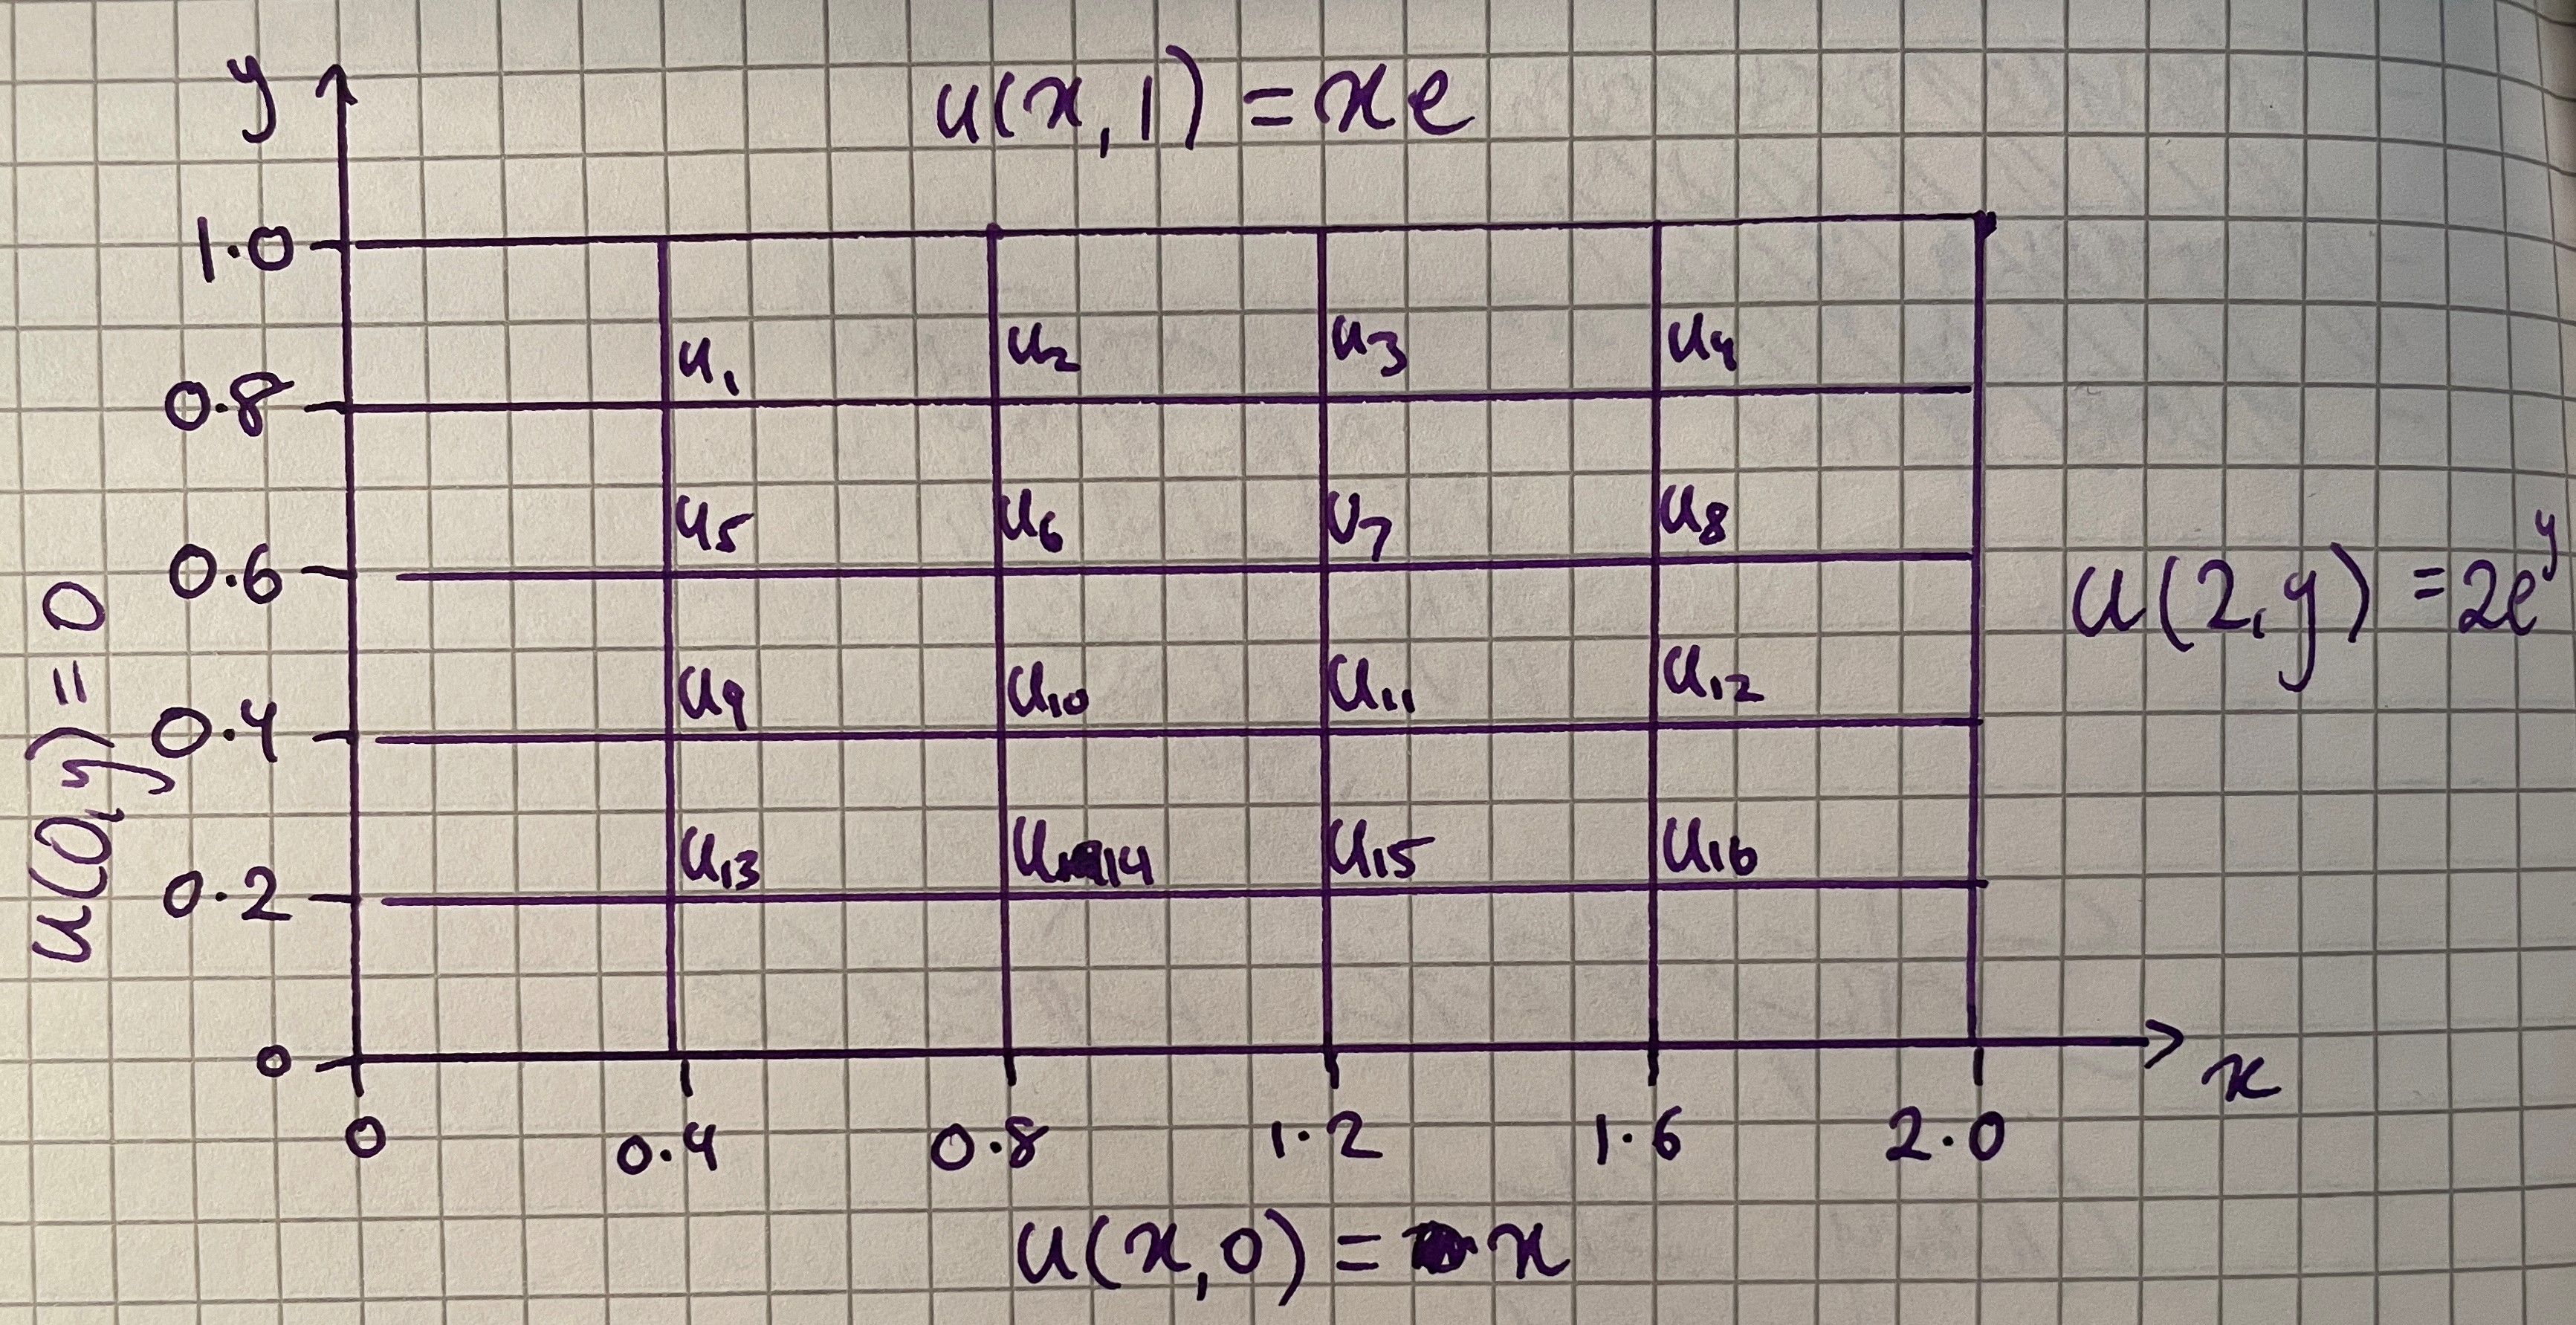
\includegraphics[width = 0.9\textwidth]{./img/q2b.JPG}
	\caption{}
\end{figure}
16 difference equations:
\begin{gather}
	10u_1 = u_2 + 0 + 4(0.4)e + 4u_5 - 0.16(0.4)e^{0.8}\\
	-10u_1 + u_2 + 4u_5 = 0.064e^{0.8} -1.6e
\end{gather} 
\begin{gather}
	10u_2 = u_3 + u_1 + 4(0.8)e + 4u_6 - 0.16(0.8)e^{0.8}\\
	-10u_2 + u_3 + u_1 + 4u_6 = 0.128e^{0.8} - 3.2e
\end{gather}
\begin{gather}
	10u_3 = u_4 + u_2 + 4(1.2)e + 4u_7 - 0.16(1.2)e^{0.8}\\
	-10u_3 + u_4 + u_2 + 4u_7 = 0.192e^{0.8} - 4.8e
\end{gather}
\begin{gather}
	10u_4 = 2e^{0.8} + u_3 + 4(1.6)e + 4u_8 - 0.16(1.6)e^{0.8}\\
	-10u_4 + u_3 + 4u_8 = -1.744e^{0.8} - 6.4e
\end{gather}
\begin{align}
	10u_5 = u_6 + 0 + 4u_1 + 4u_9 -0.16(0.4)e^{0.6}\\
	-10u_5 + u_6 + 4u_1 + 4u_9 =0.064e^{0.6}
\end{align}
\begin{align}
	10u_6 = u_7 + u_5 +4u_2 +4u_{10} -0.16(0.8)e^{0.6}\\
	-10u_6 + u_7 + u_5 + 4u_2 + 4u_{10} =0.128e^{0.6}
\end{align}
\begin{align}
	10u_7 = u_8 + u_6 + 4u_3 + 4u_{11} = 0.16(1.2)e^{0.6}\\
	-10u_7 + u_8 + u_6 + 4u_3 + 4u_{11} = 0.192e^{0.6}
\end{align}
\begin{align}
	10u_8 = 2e^{0.6} + u_7 + 4u_4 +4u_{12} -0.16(1.6)e^{0.6}\\
	-10u_8 + u_7 + 4u_4 + 4u_{12} = -1.744e^{0.6}
\end{align}
\begin{align}
	10u_9 = u_{10} + 0 + 4u_5 + 4u_{13} -0.16(0.4)e^{0.4}\\
	-10u_9 + u_{10} + 4u_5 + 4u_{13} = 0.064e^{0.4}
\end{align}
\begin{align}
	10u_{10} = u_{11} + u_9 + 4u_6 + 4u_{14}-0.16(0.8)e^{0.4}\\
	-10u_{10} + u_{11} +u_9 + 4u_{6} + 4u_{14} = 0.128e^{0.4}
\end{align}
\begin{align}
	10u_{11} = u_{12} + u_{10} + 4u_7 + 4u_{15} -0.16(1.2)e^{0.4}\\
	-10u_{11} + u_{12} + u_{10} + 4u_7 + 4u_{15} = 0.192e^{0.4}
\end{align}
\begin{align}
	10u_{12} = 2e^{0.4} + u_{11} + 4u_8 + 4u_{16} -0.16(1.6)e^{0.4}\\
	-10u_{12} + u_{11} + 4u_8 + 4u_{16} = -1.744e^{0.4}
\end{align}
\begin{align}
	10u_{13} = u_{14} + 0 + 4u_9 + 4(0.4) = 0.16(0.4)e^{0.2}\\
	-10u_{13} + u_{14} + 4u_9 = 0.064e^{0.2} - 1.6
\end{align}
\begin{align}
	10u_{14} = u_{15} + u_{13} + 4u_{10} + 4(0.8) -0.16(0.8)e^{0.2}\\
	-10u_{14} + u_{15} + u_{13} + 4u_{10} = 0.128e^{0.2}-3.2
\end{align}
\begin{align}
	10u_{15} = u_{16} + u_{14} + 4u_{11} + 4(1.2) = 0.16(1.2)e^{0.2}\\
	-10u_{15} + u_{16} + u_{14} + 4u_{11} = 0.192e^{0.2} - 4.8
\end{align}
\begin{align}
	10u_{16} = 2e^{0.2} + u_{15} + 4u_{12} + 4(1.6) -0.16(1.6)e^{0.2}\\
	-10u_{16} + u_{15} + 4u_{12} = -1.744e^{0.2} - 6.4
\end{align}

\newpage
\subsubsection*{iv \& v}
MATLAB code used to solve the system of equations above.
\lstset{language=Matlab,%
    %basicstyle=\color{red},
    breaklines=true,%
    morekeywords={matlab2tikz},
    keywordstyle=\color{blue},%
    morekeywords=[2]{1}, keywordstyle=[2]{\color{black}},
    identifierstyle=\color{black},%
    stringstyle=\color{mylilas},
    commentstyle=\color{mygreen},%
    showstringspaces=false,%without this there will be a symbol in the places where there is a space
    numbers=left,%
    numberstyle={\tiny \color{black}},% size of the numbers
    numbersep=9pt, % this defines how far the numbers are from the text
    emph=[1]{for,end,break},emphstyle=[1]\color{red}, %some words to emphasise
    %emph=[2]{word1,word2}, emphstyle=[2]{style},    
}
\lstinputlisting{Question2Code.m}
The values for the variables $w$, $wE$ and $d$ are shown below.
\begin{table}[H]
\centering
\label{q2bvals}
	\begin{tabular}{||c|c|c||} 
	\hline
	$w$ & $wE$ & $d\cdot 10^{4}$\\
	\hline
	\hline
	0.8904 & 0.8902 & 1.9117\\
	1.7808 & 1.7804 & 3.7120\\
	2.6711 & 2.6706 & 5.1109\\
	3.5613 & 3.5609 & 5.1313\\
	0.7291 & 0.7288 & 2.6628\\
	1.4582 & 1.4577 & 5.1474\\
	2.1872 & 2.1865 & 7.0008\\
	2.9160 & 2.9154 & 6.7963\\
	0.5969 & 0.5967 & 2.4853\\
	1.1939 & 1.1935 & 4.7943\\
	1.7908 & 1.7902 & 6.4859\\
	2.3875 & 2.3869 & 6.2168\\
	0.4887 & 0.4886 & 1.5553\\
	0.9774 & 0.9771 & 3.0022\\
	1.4660 & 1.4657 & 4.0711\\
	1.9546 & 1.9542 & 3.9375\\
	\hline
 \end{tabular}
 \caption{Values for $w$, $wE$ and $d$.}
\end{table}
As seen in the table above, our error term is on the magnitude of $10^{-4}$ which is a relatively tiny error. Hence, our approximation is useful.
\end{document}